% answers.tex —— 2011 年·山东卷·理科 · 参考答案与详细解析片段
% 由 tools/generate_projects.py 依来源总账自 2011/2011_数学真题_山东理_试题.md + 2011/2011_数学真题_山东理_解析正文.md + 2011/2011_数学真题_山东理_答案要点.md 生成，勿手改（改源 MD 后重跑）

\begin{answer}
\gksolhead{1}{}

\textbf{题目}：

设集合 $M=\{x\mid x^2+x-6<0\}$，$N=\{x\mid 1\leqslant x\leqslant 3\}$，则 $M\cap N=$\mbox{（　　）}

（A）$[1,2)$

（B）$[1,2]$

（C）$(2,3]$

（D）$[2,3]$

\Needspace{4\baselineskip}
\textbf{解析}
\Needspace{5\baselineskip}
$M$ 即 $x^2+x-6<0$，因式分解 $(x+3)(x-2)<0$，得 $M=(-3,2)$；$N=[1,3]$。故
\nopagebreak[4]
\[M\cap N=[1,2).\]
逐项排除：（B）把右端点误作闭；（C）把左端点误取 $2$；（D）把交集误作 $N$ 的前段。

\gkanswer{答案：A。}

\end{answer}
\begin{answer}
\gksolhead{2}{}

\textbf{题目}：

复数 $z=\dfrac{2-\mathrm i}{2+\mathrm i}$（$\mathrm i$ 为虚数单位）在复平面内对应的点所在的象限为\mbox{（　　）}

（A）第一象限

（B）第二象限

（C）第三象限

（D）第四象限

\Needspace{4\baselineskip}
\textbf{解析}
\Needspace{5\baselineskip}
分子分母同乘 $2-\mathrm i$：
\nopagebreak[4]
\[z=\frac{(2-\mathrm i)^2}{(2+\mathrm i)(2-\mathrm i)}=\frac{4-4\mathrm i+\mathrm i^2}{5}=\frac{3-4\mathrm i}{5}.\]
实部 $\dfrac35>0$、虚部 $-\dfrac45<0$，对应点在第四象限。选 D。

\gkanswer{答案：D。}

\end{answer}
\begin{answer}
\gksolhead{3}{}

\textbf{题目}：

若点 $(a,9)$ 在函数 $y=3^x$ 的图象上，则 $\tan\dfrac{a\pi}{6}$ 的值为\mbox{（　　）}

（A）$0$

（B）$\frac{\sqrt3}{3}$

（C）$1$

（D）$\sqrt3$

\Needspace{4\baselineskip}
\textbf{解析}
$3^a=9=3^2$，故 $a=2$，$\tan\dfrac{2\pi}{6}=\tan\dfrac\pi3=\sqrt3$。选 D。

\gkanswer{答案：D。}

\end{answer}
\begin{answer}
\gksolhead{4}{}

\textbf{题目}：

不等式 $|x-5|+|x+3|\geqslant10$ 的解集是\mbox{（　　）}

（A）$[-5,7]$

（B）$[-4,6]$

（C）$(-\infty,-5]\cup[7,+\infty)$

（D）$(-\infty,-4]\cup[6,+\infty)$

\Needspace{4\baselineskip}
\textbf{解析}
令 $g(x)=|x-5|+|x+3|$。当 $-3\leqslant x\leqslant5$ 时 $g(x)=8<10$；当 $x>5$ 时 $g(x)=2x-2\geqslant10$ 得 $x\geqslant6$；当 $x<-3$ 时 $g(x)=-2x+2\geqslant10$ 得 $x\leqslant-4$。故解集为 $(-\infty,-4]\cup[6,+\infty)$，选 D。

\gkanswer{答案：D。}

\end{answer}
\begin{answer}
\gksolhead{5}{}

\textbf{题目}：

对于函数 $y=f(x)$，$x\in\mathbf R$。“$y=|f(x)|$ 的图象关于 $y$ 轴对称”是“$y=f(x)$ 是奇函数”的\mbox{（　　）}

（A）充分而不必要条件

（B）必要而不充分条件

（C）充要条件

（D）既不充分也不必要条件

\Needspace{4\baselineskip}
\textbf{解析}
若 $f$ 为奇函数，则 $|f(-x)|=|-f(x)|=|f(x)|$，$|f(x)|$ 为偶函数，图象关于 $y$ 轴对称，故条件是必要的。反之，取 $f(x)=x^2$，$|f(x)|=x^2$ 关于 $y$ 轴对称，但 $f$ 不是奇函数，故不充分。因此是必要而不充分条件，选 B。

\gkanswer{答案：B。}

\end{answer}
\begin{answer}
\gksolhead{6}{}

\textbf{题目}：

若函数 $f(x)=\sin\omega x$（$\omega>0$）在区间 $\left[0,\dfrac{\pi}{3}\right]$ 上单调递增，在区间 $\left[\dfrac{\pi}{3},\dfrac{\pi}{2}\right]$ 上单调递减，则 $\omega=$\mbox{（　　）}

（A）$3$

（B）$2$

（C）$\frac32$

（D）$\frac23$

\Needspace{4\baselineskip}
\textbf{解析}
$\sin\omega x$ 在 $x=\dfrac{\pi}{3}$ 处取最大值，故 $\omega\cdot\dfrac\pi3=\dfrac\pi2+2k\pi$。又 $\omega>0$ 且在 $\left[0,\dfrac\pi3\right]$ 上递增、在 $\left[\dfrac\pi3,\dfrac\pi2\right]$ 上递减，取最小正周期对应 $k=0$，得 $\omega=\dfrac32$。选 C。

\gkanswer{答案：C。}

\end{answer}
\begin{answer}
\gksolhead{7}{}

\textbf{题目}：

某产品的广告费用 $x$ 与销售额 $y$ 的统计数据如下表：

\begin{center}
\begin{tabular}{lllll}
\toprule
广告费用 $x$（万元） & 4 & 2 & 3 & 5 \\
\midrule
销售额 $y$（万元） & 49 & 26 & 39 & 54 \\
\bottomrule
\end{tabular}
\end{center}

根据上表可得回归方程 $\hat y=\hat bx+\hat a$ 中的 $\hat b$ 为 $9.4$，据此模型预报广告费用为 $6$ 万元时销售额为\mbox{（　　）}

（A）$63.6$ 万元

（B）$65.5$ 万元

（C）$67.7$ 万元

（D）$72.0$ 万元

\Needspace{4\baselineskip}
\textbf{解析}
$\bar x=\dfrac{4+2+3+5}{4}=3.5$，$\bar y=\dfrac{49+26+39+54}{4}=42$。由 $\bar y=\hat b\bar x+\hat a$ 得 $\hat a=42-9.4\times3.5=42-32.9=9.1$。$x=6$ 时 $\hat y=9.4\times6+9.1=65.5$（万元）。选 B。

\gkanswer{答案：B。}

\end{answer}
\begin{answer}
\gksolhead{8}{}

\textbf{题目}：

已知双曲线 $\dfrac{x^2}{a^2}-\dfrac{y^2}{b^2}=1$（$a>0$，$b>0$）的两条渐近线均和圆 $C:x^2+y^2-6x+5=0$ 相切，且双曲线的右焦点为圆 $C$ 的圆心，则该双曲线的方程为\mbox{（　　）}

（A）$\frac{x^2}{5}-\frac{y^2}{4}=1$

（B）$\frac{x^2}{4}-\frac{y^2}{5}=1$

（C）$\frac{x^2}{3}-\frac{y^2}{6}=1$

（D）$\frac{x^2}{6}-\frac{y^2}{3}=1$

\Needspace{4\baselineskip}
\textbf{解析}
\Needspace{5\baselineskip}
圆 $C:x^2+y^2-6x+5=0$ 即 $(x-3)^2+y^2=4$，圆心 $(3,0)$、半径 $2$。右焦点为 $(3,0)$，故 $c=3$。渐近线 $bx\pm ay=0$ 与圆相切：
\nopagebreak[4]
\[\frac{|3b|}{\sqrt{a^2+b^2}}=2\Longrightarrow 9b^2=4(a^2+b^2)=4c^2=36,\]
故 $b^2=4$，$a^2=c^2-b^2=5$。双曲线为 $\dfrac{x^2}{5}-\dfrac{y^2}{4}=1$，选 A。

\gkanswer{答案：A。}

\end{answer}
\begin{answer}
\gksolhead{9}{}

\textbf{题目}：

函数 $y=\dfrac x2-2\sin x$ 的图象大致是\mbox{（　　）}

（A）图 A

（B）图 B

（C）图 C

（D）图 D
\nopagebreak[4]
\begin{center}% 2011 年山东卷理科第 9 题：四个选项的函数图象（选项图）。
% 来源 PDF：普通高考/2011/2011山东理.pdf，SHA-256 d0f409fd3fa82b12c210d587c8412d4c446946a201f87d124e2fc17c5a50db16。
% 原页：第 1 页（A3 三栏）第 1 栏下部接第 2 栏上部，书页码 689。
% 重绘依据：原页四图为示意图，纵轴「4」刻度与横轴「2π」刻度的实际比例与 y=x/2-2sin x
%   的取值并不一致（原页纵向压缩），故按 600 dpi 逐像素提取曲线拓扑后重绘，刻度位置照原页：
%   (A) 曲线形如 y=0.31x-1.24cos x（含偶函数项，不关于原点对称，左支与右支不同号）；
%   (B) 曲线形如 y=0.61x-1.84sin x（奇函数，振幅相对一次项小，|x|>4 出图）；
%   (C) 曲线形如 y=0.31x-1.26sin x，与 y=(x/2-2sin x) 同形（零点 ±2.475，极值 x≈±1.32、±4.97、±7.60）；
%   (D) 为奇函数曲线，小极值在 x≈±1.5、大极值在 x≈±6.6，按原页数字化控制点平滑重绘。
%   四图的坐标轴、箭头、刻度「4」「2π」与「O」的位置均照原页，不按比例。
\begin{tikzpicture}[>=stealth, semithick, font=\small, x=0.17cm, y=0.28cm]

  % ================= (A) =================
  \begin{scope}
    \draw[->] (-12.1,0) -- (12.2,0) node[right] {$x$};
    \draw[->] (0,-4.35) -- (0,4.30) node[above] {$y$};
    \draw (-2.4,4) -- (2.4,4);
    \node[left] at (-2.6,4) {$4$};
    \draw (6.283,-0.22) -- (6.283,0.22);
    \node[below] at (6.283,-0.22) {$2\pi$};
    \node at (-2.4,-1.5) {$O$};
    \draw[thick, domain=-10.1:10.1, samples=280]
      plot (\x, {0.31*\x - 1.24*cos(\x r)});
    \node at (-6.4,-6.2) {(A)};
  \end{scope}

  % ================= (B) =================
  \begin{scope}[xshift=7.6cm]
    \draw[->] (-12.1,0) -- (12.2,0) node[right] {$x$};
    \draw[->] (0,-4.35) -- (0,4.30) node[above] {$y$};
    \draw (-2.4,4) -- (2.4,4);
    \node[left] at (-2.6,4) {$4$};
    \draw (6.283,-0.22) -- (6.283,0.22);
    \node[below] at (6.283,-0.22) {$2\pi$};
    \node at (-2.4,-1.5) {$O$};
    \draw[thick, domain=-4.1:4.1, samples=200]
      plot (\x, {0.61*\x - 1.84*sin(\x r)});
    \node at (-6.4,-6.2) {(B)};
  \end{scope}

  % ================= (C) =================
  \begin{scope}[yshift=-6.6cm]
    \draw[->] (-12.1,0) -- (12.2,0) node[right] {$x$};
    \draw[->] (0,-4.35) -- (0,4.30) node[above] {$y$};
    \draw (-2.4,4) -- (2.4,4);
    \node[left] at (-2.6,4) {$4$};
    \draw (6.283,-0.22) -- (6.283,0.22);
    \node[below] at (6.283,-0.22) {$2\pi$};
    \node at (-2.4,-1.5) {$O$};
    \draw[thick, domain=-10.1:10.1, samples=280]
      plot (\x, {0.31*\x - 1.26*sin(\x r)});
    \node at (-6.4,-6.2) {(C)};
  \end{scope}

  % ================= (D) =================
  \begin{scope}[xshift=7.6cm, yshift=-6.6cm]
    \draw[->] (-12.1,0) -- (12.2,0) node[right] {$x$};
    \draw[->] (0,-4.35) -- (0,4.30) node[above] {$y$};
    \draw (-2.4,4) -- (2.4,4);
    \node[left] at (-2.6,4) {$4$};
    \draw (6.283,-0.22) -- (6.283,0.22);
    \node[below] at (6.283,-0.22) {$2\pi$};
    \node at (-2.4,-1.5) {$O$};
    \draw[thick] plot[smooth, tension=0.75] coordinates {
      (-10.08,3.42) (-9.58,2.00) (-8.57,-0.70) (-7.57,-2.38) (-6.55,-2.78)
      (-5.55,-2.20) (-4.53,-1.21) (-3.53,-0.11) (-2.52,0.90) (-1.52,1.30)
      (-0.50,0.70) (0.15,0.20) (0,0) (-0.15,-0.20) (0.50,-0.71)
      (1.52,-1.31) (2.52,-0.90) (3.53,0.11) (4.53,1.21) (5.55,2.20)
      (6.55,2.78) (7.56,2.39) (8.57,0.68) (9.58,-2.02) (10.08,-3.42)};
    \node at (-6.4,-6.2) {(D)};
  \end{scope}

\end{tikzpicture}
\end{center}
\nopagebreak[4]
\Needspace{4\baselineskip}
\textbf{解析}
$f(x)=\dfrac x2-2\sin x$ 为奇函数，图象关于原点对称。$f'(x)=\dfrac12-2\cos x$，$f'(0)=-\dfrac32<0$，故 $x>0$ 很小时 $f(x)<0$，曲线从原点向右下方进入第四象限；$f(2\pi)=\pi>0$，曲线在 $x=2\pi$ 处已回到 $x$ 轴上方。结合周期内的增减与极值位置，只有（C）符合。选 C。

\gkanswer{答案：C。}

\end{answer}
\begin{answer}
\gksolhead{10}{}

\textbf{题目}：

已知 $f(x)$ 是 $\mathbf R$ 上最小正周期为 $2$ 的周期函数，且当 $0\leqslant x<2$ 时，$f(x)=x^3-x$，则函数 $y=f(x)$ 的图象在区间 $[0,6]$ 上与 $x$ 轴的交点的个数为\mbox{（　　）}

（A）$6$

（B）$7$

（C）$8$

（D）$9$

\Needspace{4\baselineskip}
\textbf{解析}
在 $[0,2)$ 上 $f(x)=x(x-1)(x+1)$，零点为 $0,1$。由周期 $2$，在 $[2,4)$、$[4,6)$ 上零点分别为 $2,3$ 与 $4,5$；端点 $6$ 也是零点。共 $0,1,2,3,4,5,6$ 七个，选 B。

\gkanswer{答案：B。}

\end{answer}
\begin{answer}
\gksolhead{11}{}

\textbf{题目}：

如图是长和宽分别相等的两个矩形。给定下列三个命题：① 存在三棱柱，其正（主）视图、俯视图如图；② 存在四棱柱，其正（主）视图、俯视图如图；③ 存在圆柱，其正（主）视图、俯视图如图。其中真命题的个数是\mbox{（　　）}

（A）$3$

（B）$2$

（C）$1$

（D）$0$
\nopagebreak[4]
\begin{center}% 2011 年山东卷理科第 11 题：两个全等矩形的正（主）视图与俯视图。
% 来源 PDF：普通高考/2011/2011山东理.pdf，SHA-256 d0f409fd3fa82b12c210d587c8412d4c446946a201f87d124e2fc17c5a50db16。
% 原页：第 1 页（A3 三栏）第 2 栏中部，书页码 689。
% 重绘依据：照原页——左、右两个同样大小（长宽比约 5:3）的矩形并排，图上无尺寸标注，
%   仅在下方分别标「正（主）视图」「俯视图」；两矩形外框为各自视图的轮廓，不画投影连线。
\begin{tikzpicture}[scale=1.0, semithick]
  \draw (0,0) rectangle (2.4,1.45);
  \node[below] at (1.2,-0.12) {正（主）视图};
  \draw (3.3,0) rectangle (5.7,1.45);
  \node[below] at (4.5,-0.12) {俯视图};
\end{tikzpicture}
\end{center}
\nopagebreak[4]
\Needspace{4\baselineskip}
\textbf{解析}
三个命题都可实现：① 取横放的三棱柱，使一个矩形侧面正对观察者，正视图为矩形、俯视图也为矩形；② 取长方体（四棱柱），正视图与俯视图均为矩形；③ 取横放的圆柱，并使其长等于底面直径，则正视图与俯视图都是同样长宽的矩形。故真命题有 $3$ 个，选 A。

\gkanswer{答案：A。}

\end{answer}
\begin{answer}
\gksolhead{12}{}

\textbf{题目}：

设 $A_1$，$A_2$，$A_3$，$A_4$ 是平面直角坐标系中两两不同的四点，若 $\overrightarrow{A_1A_3}=\lambda\overrightarrow{A_1A_2}$（$\lambda\in\mathbf R$），$\overrightarrow{A_1A_4}=\mu\overrightarrow{A_1A_2}$（$\mu\in\mathbf R$），且 $\dfrac1\lambda+\dfrac1\mu=2$，则称 $A_3$，$A_4$ 调和分割 $A_1$，$A_2$。已知平面上的点 $C$，$D$ 调和分割点 $A$，$B$，则下面说法正确的是\mbox{（　　）}

（A）$C$ 可能是线段 $AB$ 的中点

（B）$D$ 可能是线段 $AB$ 的中点

（C）$C$，$D$ 可能同时在线段 $AB$ 上

（D）$C$，$D$ 不可能同时在线段 $AB$ 的延长线上

\Needspace{4\baselineskip}
\textbf{解析}
设 $\overrightarrow{AB}=\boldsymbol b$，则 $C=A+\lambda\boldsymbol b$，$D=A+\mu\boldsymbol b$，且 $\dfrac1\lambda+\dfrac1\mu=2$。
若 $C$ 为 $AB$ 中点，$\lambda=\dfrac12$，则 $\dfrac1\mu=0$，无解，A 错；同理 B 错。
若 $C,D$ 都在线段 $AB$ 上，则 $0<\lambda,\mu<1$，$\dfrac1\lambda+\dfrac1\mu>2$，C 错。
若 $C,D$ 都在 $AB$ 的延长线上：同向延长时 $\lambda,\mu>1$，倒数和小于 $2$；分别在两侧时一正一负，倒数和小于 $1$。均不可能，故 D 正确。选 D。

\gkanswer{答案：D。}

\end{answer}
\begin{answer}
\gksolhead{13}{}

\textbf{题目}：

执行如图所示的程序框图，输入 $l=2$，$m=3$，$n=5$，则输出的 $y$ 的值是 $\underline{\qquad}$。
\nopagebreak[4]
\begin{center}% 2011 年山东卷理科第 13 题：程序框图。
% 来源 PDF：普通高考/2011/2011山东理.pdf，SHA-256 d0f409fd3fa82b12c210d587c8412d4c446946a201f87d124e2fc17c5a50db16。
% 原页：第 1 页（A3 三栏）第 2 栏下部，书页码 689。
% 重绘依据：照原页——自上而下「开始」→ 平行四边形「输入非负整数 l, m, n」→
%   菱形「l^2+m^2+n^2=0?」：「是」向左下到矩形「y=105」，「否」向下到矩形「y=70l+21m+15n」；
%   再由菱形「y>105?」判断：「是」向右到矩形「y=y-105」并回折上行，汇入「y>105?」上方的竖线；
%   「否」向下经平行四边形「输出 y」到「结束」。y=105 支路的连线向右汇入「输出 y」上方的竖线。
\begin{tikzpicture}[>=stealth, semithick, font=\small]
  \node[draw, rounded corners=0.12cm, minimum width=1.2cm, minimum height=0.5cm] (start) at (0,0) {开始};
  \node[draw, trapezium, trapezium left angle=72, trapezium right angle=108,
        minimum width=3.5cm, minimum height=0.55cm] (input) at (0,-1.15) {输入非负整数 $l$，$m$，$n$};
  \node[draw, diamond, aspect=1.7, minimum width=3.0cm, minimum height=0.95cm] (test1) at (0,-2.55) {$l^2+m^2+n^2=0$};
  \node[draw, minimum width=1.5cm, minimum height=0.55cm] (y105) at (-3.5,-4.15) {$y=105$};
  \node[draw, minimum width=3.4cm, minimum height=0.55cm] (yval) at (0,-4.15) {$y=70l+21m+15n$};
  \node[draw, diamond, aspect=1.7, minimum width=3.0cm, minimum height=0.95cm] (test2) at (0,-5.85) {$y>105$};
  \node[draw, minimum width=2.2cm, minimum height=0.55cm] (dec) at (4.0,-5.85) {$y=y-105$};
  \node[draw, trapezium, trapezium left angle=72, trapezium right angle=108,
        minimum width=1.8cm, minimum height=0.55cm] (out) at (0,-7.3) {输出 $y$};
  \node[draw, rounded corners=0.12cm, minimum width=1.2cm, minimum height=0.5cm] (stop) at (0,-8.4) {结束};
  % 主干
  \draw[->] (start.south) -- (input.north);
  \draw[->] (input.south) -- (test1.north);
  \draw[->] (test1.east) -| (yval.north) node[pos=0.25, right] {否};
  \draw[->] (yval.south) -- (test2.north);
  \draw[->] (test2.south) -- (out.north) node[midway, right] {否};
  \draw[->] (out.south) -- (stop.north);
  % 「是」支路：左侧 y=105，向下汇入「输出 y」上方的竖线
  \draw[->] (test1.west) -| (y105.north) node[pos=0.25, above] {是};
  \draw (y105.south) -- (y105.south |- out.north) -- (out.north);
  % 回环：y=y-105 向左汇入「y>105?」上方竖线
  \draw[->] (test2.east) -- (dec.west) node[midway, above] {是};
  \draw (dec.north) -- (4.0,-4.75) -- (0,-4.75);
\end{tikzpicture}
\end{center}
\nopagebreak[4]
\Needspace{4\baselineskip}
\textbf{解析}
$l^2+m^2+n^2=4+9+25=38\neq0$，先取 $y=70l+21m+15n=140+63+75=278$。$278>105$，减去 $105$ 得 $173$；$173>105$，再减得 $68$；$68\leqslant105$，输出 $y=68$。

\gkanswer{答案：$68$。}

\end{answer}
\begin{answer}
\gksolhead{14}{}

\textbf{题目}：

若 $\left(x-\dfrac{\sqrt a}{x^2}\right)^6$ 展开式的常数项为 $60$，则常数 $a$ 的值为 $\underline{\qquad}$。

\Needspace{4\baselineskip}
\textbf{解析}
\Needspace{5\baselineskip}
通项
\nopagebreak[4]
\[\mathrm C_6^k x^{6-k}\left(-\frac{\sqrt a}{x^2}\right)^k=\mathrm C_6^k(-\sqrt a)^k x^{6-3k}.\]
常数项要求 $6-3k=0$，即 $k=2$，故 $\mathrm C_6^2a=15a=60$，$a=4$。

\gkanswer{答案：$4$。}

\end{answer}
\begin{answer}
\gksolhead{15}{}

\textbf{题目}：

\Needspace{5\baselineskip}
设函数 $f(x)=\dfrac{x}{x+2}$（$x>0$），观察：
\nopagebreak[4]
\[f_1(x)=f(x)=\frac{x}{x+2},\]
\nopagebreak[4]
\[f_2(x)=f(f_1(x))=\frac{x}{3x+4},\]
\nopagebreak[4]
\[f_3(x)=f(f_2(x))=\frac{x}{7x+8},\]
\nopagebreak[4]
\[f_4(x)=f(f_3(x))=\frac{x}{15x+16},\]
\nopagebreak[4]
\[\cdots\]
根据以上事实，由归纳推理可得：当 $n\in\mathbf N^*$ 且 $n\geqslant2$ 时，$f_n(x)=f(f_{n-1}(x))=$ $\underline{\qquad}$。

\Needspace{4\baselineskip}
\textbf{解析}
\Needspace{5\baselineskip}
观察分母：$f_1$ 为 $x+2$，$f_2$ 为 $3x+4$，$f_3$ 为 $7x+8$，$f_4$ 为 $15x+16$，即 $f_n$ 的分母为 $(2^n-1)x+2^n$。验证递推：
\nopagebreak[4]
\[f(f_{n-1}(x))=\frac{\dfrac{x}{(2^{n-1}-1)x+2^{n-1}}}{\dfrac{x}{(2^{n-1}-1)x+2^{n-1}}+2}
=\frac{x}{(2^n-1)x+2^n}.\]
故 $f_n(x)=\dfrac{x}{(2^n-1)x+2^n}$。

\gkanswer{答案：$\dfrac{x}{(2^n-1)x+2^n}$。}

\end{answer}
\begin{answer}
\gksolhead{16}{}

\textbf{题目}：

已知函数 $f(x)=\log_ax+x-b$（$a>0$，且 $a\neq1$）。当 $2<a<3<b<4$ 时，函数 $f(x)$ 的零点 $x_0\in(n,n+1)$，$n\in\mathbf N^*$，则 $n=$ $\underline{\qquad}$。

\Needspace{4\baselineskip}
\textbf{解析}
$f(2)=\log_a2+2-b$。因 $2<a<3$ 得 $0<\log_a2<1$，又 $b>3$，故 $f(2)<1+2-3=0$。
$f(3)=\log_a3+3-b$。因 $a<3$ 得 $\log_a3>1$，又 $b<4$，故 $f(3)>1+3-4=0$。
$f$ 在 $(0,+\infty)$ 上单调递增，故唯一零点 $x_0\in(2,3)$，$n=2$。

\gkanswer{答案：$2$。}

\end{answer}
\begin{answer}
\gksolhead{17}{}

\textbf{题目}：

在 $\triangle ABC$ 中，内角 $A$，$B$，$C$ 的对边分别为 $a$，$b$，$c$，已知 $\dfrac{\cos A-2\cos C}{\cos B}=\dfrac{2c-a}{b}$。

（1） 求 $\dfrac{\sin C}{\sin A}$ 的值；

（2） 若 $\cos B=\dfrac14$，$b=2$，求 $\triangle ABC$ 的面积 $S$。

\Needspace{4\baselineskip}
\textbf{解析}
\gksubpart{(1)}
\Needspace{5\baselineskip}
由正弦定理，$\dfrac{2c-a}{b}=\dfrac{2\sin C-\sin A}{\sin B}$。条件即
\nopagebreak[4]
\[\frac{\cos A-2\cos C}{\cos B}=\frac{2\sin C-\sin A}{\sin B}.\]
\Needspace{5\baselineskip}
去分母：
\nopagebreak[4]
\[\sin B\cos A-2\sin B\cos C=2\sin C\cos B-\sin A\cos B,\]
\Needspace{5\baselineskip}
移项得
\nopagebreak[4]
\[\sin B\cos A+\sin A\cos B=2(\sin C\cos B+\sin B\cos C),\]
即 $\sin(A+B)=2\sin(B+C)$。因 $A+B=\pi-C$，$B+C=\pi-A$，故 $\sin C=2\sin A$，$\dfrac{\sin C}{\sin A}=2$。

\gksubpart{(2)}
\Needspace{5\baselineskip}
由（1） $c=2a$。由余弦定理
\nopagebreak[4]
\[b^2=a^2+c^2-2ac\cos B=a^2+4a^2-4a^2\cdot\frac14=4a^2,\]
\Needspace{5\baselineskip}
故 $a=1$，$c=2$。$\sin B=\sqrt{1-\dfrac1{16}}=\dfrac{\sqrt{15}}4$，面积
\nopagebreak[4]
\[S=\frac12ac\sin B=\frac12\cdot1\cdot2\cdot\frac{\sqrt{15}}4=\frac{\sqrt{15}}4.\]

\gkanswer{答案（1）：$2$。}

\gkanswer{答案（2）：$\dfrac{\sqrt{15}}{4}$。}

\end{answer}
\begin{answer}
\gksolhead{18}{}

\textbf{题目}：

红队队员甲、乙、丙与蓝队队员 $A$、$B$、$C$ 进行围棋比赛，甲对 $A$、乙对 $B$、丙对 $C$ 各一盘。已知甲胜 $A$、乙胜 $B$、丙胜 $C$ 的概率分别为 $0.6$，$0.5$，$0.5$，假设各盘比赛结果相互独立。

（1） 求红队至少两名队员获胜的概率；

（2） 用 $\xi$ 表示红队队员获胜的总盘数，求 $\xi$ 的分布列和数学期望 $E\xi$。

\Needspace{4\baselineskip}
\textbf{解析}
记甲、乙、丙获胜分别为事件 $A_1,A_2,A_3$，概率 $0.6,0.5,0.5$，相互独立。

\gksubpart{(1)}
\Needspace{5\baselineskip}
至少两人获胜 = 恰两人 + 三人全胜：
\nopagebreak[4]
\[0.6\times0.5\times0.5+0.6\times0.5\times0.5+0.4\times0.5\times0.5+0.6\times0.5\times0.5=0.15+0.15+0.10+0.15=0.55.\]

\gksubpart{(2)}
逐个基本事件求和：
$P(\xi=0)=0.4\times0.5\times0.5=0.1$；
$P(\xi=1)=0.6\times0.5\times0.5+0.4\times0.5\times0.5+0.4\times0.5\times0.5=0.15+0.1+0.1=0.35$；
$P(\xi=2)=0.4$（由（1）恰两人）；
$P(\xi=3)=0.15$。
故分布列为
\begin{center}
\begin{tabular}{lllll}
\toprule
$\xi$ & 0 & 1 & 2 & 3 \\
\midrule
$P$ & 0.1 & 0.35 & 0.4 & 0.15 \\
\bottomrule
\end{tabular}
\end{center}

$E\xi=0\times0.1+1\times0.35+2\times0.4+3\times0.15=0.35+0.8+0.45=1.6$。

\gkanswer{答案（1）：$0.55$。}

\gkanswer{答案（2）：$P(\xi=0)=0.1$，$P(\xi=1)=0.35$，$P(\xi=2)=0.4$，$P(\xi=3)=0.15$，$E\xi=1.6$。}

\end{answer}
\begin{answer}
\gksolhead{19}{}

\textbf{题目}：

在如图所示的几何体中，四边形 $ABCD$ 为平行四边形，$\angle ACB=90^\circ$，$EA\perp$ 平面 $ABCD$，$EF\parallel AB$，$FG\parallel BC$，$EG\parallel AC$，$AB=2EF$。

（1） 若 $M$ 是线段 $AD$ 的中点，求证：$GM\parallel$ 平面 $ABFE$；

（2） 若 $AC=BC=2AE$，求二面角 $A-BF-C$ 的大小。
\nopagebreak[4]
\begin{center}% 2011 年山东卷理科第 19 题：多面体 ABCD-EFG，AB = 2EF，EF∥AB，FG∥BC，EG∥AC，EA⊥平面 ABCD。
% 来源 PDF：普通高考/2011/2011山东理.pdf，SHA-256 d0f409fd3fa82b12c210d587c8412d4c446946a201f87d124e2fc17c5a50db16。
% 原页：第 2 页（A3 三栏）第 1 栏上部，书页码 690。
% 重绘依据：照原页作斜二测示意（AC = BC = 2AE）。经核实该多面体共有 7 个面：
%   底面 ABCD（平行四边形），面 ABFE（等腰梯形，AB∥EF 且 AB=2EF），面 ADE（三角形），
%   面 BCFG（四边形，FG∥BC），面 CDG（三角形），面 DEG（三角形），面 EFG（三角形）。
%   可见棱（实线）：BC、CD、CG、DE、DG、EF、EG、FB、FG；
%   被遮棱（虚线）：AB、AD、AE；另按原页用虚线画出底面对角线 AC（标出 ∠ACB=90°）与线段 GM（M 为 AD 中点）。
%   拓扑与原页一致，不按比例。
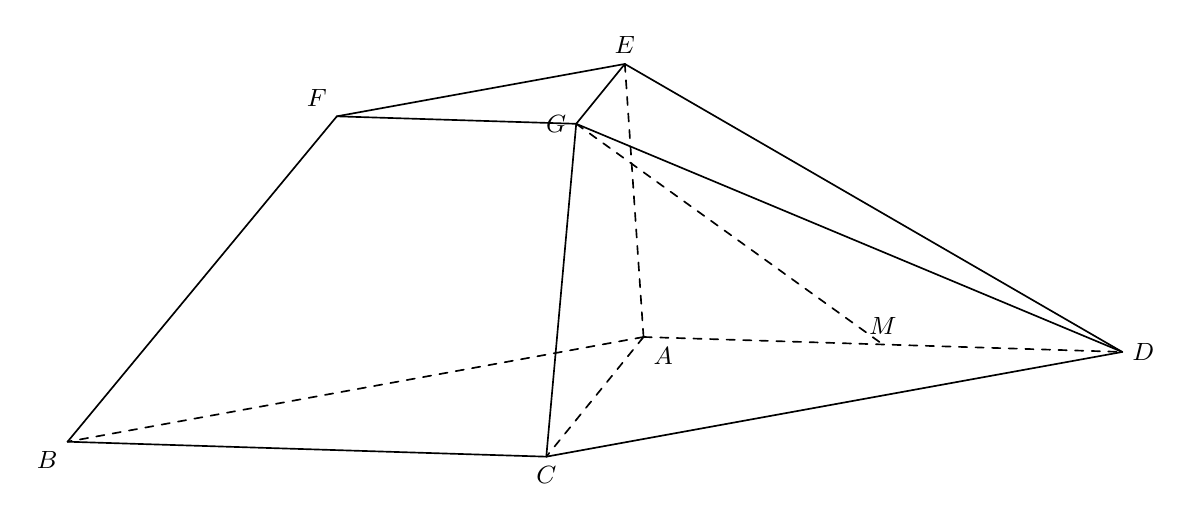
\begin{tikzpicture}[scale=0.95, >=stealth, semithick, font=\small,
  line cap=round]
  \coordinate (B) at (3.60,4.50);
  \coordinate (C) at (10.00,4.30);
  \coordinate (A) at (11.30,5.90);
  \coordinate (D) at (17.70,5.70);
  \coordinate (E) at (11.05,9.55);
  \coordinate (F) at (7.20,8.85);
  \coordinate (G) at (10.40,8.75);
  \coordinate (M) at (14.50,5.80);
  % 可见棱
  \draw (B) -- (C) -- (D);
  \draw (C) -- (G);
  \draw (D) -- (E);
  \draw (D) -- (G);
  \draw (E) -- (F);
  \draw (E) -- (G);
  \draw (F) -- (B);
  \draw (F) -- (G);
  % 被遮棱
  \draw[dashed] (A) -- (B);
  \draw[dashed] (A) -- (D);
  \draw[dashed] (A) -- (E);
  % 底面对角线 AC（原页用虚线画出，以显示 ∠ACB = 90°）
  \draw[dashed] (A) -- (C);
  % 线段 GM（M 为 AD 的中点）
  \draw[dashed] (G) -- (M);
  % 顶点标注
  \node[above] at (E) {$E$};
  \node[above left] at (F) {$F$};
  \node[left] at (G) {$G$};
  \node[below left] at (B) {$B$};
  \node[below] at (C) {$C$};
  \node[below right] at (A) {$A$};
  \node[right] at (D) {$D$};
  \node[above] at (M) {$M$};
\end{tikzpicture}
\end{center}
\nopagebreak[4]
\Needspace{4\baselineskip}
\textbf{解析}
\Needspace{5\baselineskip}
以 $C$ 为原点，$CA$ 为 $x$ 轴、$CB$ 为 $y$ 轴建立空间直角坐标系。设 $AC=BC=2$，$AE=1$，则
\nopagebreak[4]
\[C(0,0,0),\quad A(2,0,0),\quad B(0,2,0),\quad D(2,-2,0),\quad E(2,0,1).\]
由 $EF\parallel AB$、$AB=2EF$，得 $F(1,1,1)$；由 $EG\parallel AC$、$FG\parallel BC$，得 $G(1,0,1)$。

\gksubpart{(1)}
\Needspace{5\baselineskip}
$M$ 为 $AD$ 中点，$M(2,-1,0)$，故 $\overrightarrow{GM}=(1,-1,-1)$。平面 $ABFE$ 内 $\overrightarrow{AE}=(0,0,1)$，$\overrightarrow{AB}=(-2,2,0)$，法向量
\nopagebreak[4]
\[\boldsymbol n=\overrightarrow{AE}\times\overrightarrow{AB}=(-2,-2,0),\]
取 $\boldsymbol n=(1,1,0)$。于是 $\overrightarrow{GM}\cdot\boldsymbol n=1-1+0=0$，$GM\parallel$ 平面 $ABFE$。又 $M$ 不在该平面内（代入平面方程 $(x-2)+y=0$ 得 $-1\neq0$），故 $GM\parallel$ 平面 $ABFE$。

\gksubpart{(2)}
\Needspace{5\baselineskip}
平面 $ABF$ 的法向量即 $\boldsymbol n_1=(1,1,0)$。平面 $BCF$ 内 $\overrightarrow{BC}=(0,-2,0)$，$\overrightarrow{BF}=(1,-1,1)$，法向量
\nopagebreak[4]
\[\boldsymbol n_2=\overrightarrow{BC}\times\overrightarrow{BF}=(-2,0,2),\]
\Needspace{5\baselineskip}
取 $\boldsymbol n_2=(-1,0,1)$。则
\nopagebreak[4]
\[\cos\langle\boldsymbol n_1,\boldsymbol n_2\rangle=\frac{-1}{\sqrt2\cdot\sqrt2}=-\frac12,\]
两平面法向量夹角为 $120^\circ$，故二面角 $A-BF-C$ 为 $60^\circ$（即 $\dfrac\pi3$）。

\gkanswer{答案（1）：证明见解析。}

\gkanswer{答案（2）：$60^\circ$（即 $\dfrac{\pi}{3}$）。}

\end{answer}
\begin{answer}
\gksolhead{20}{}

\textbf{题目}：

等比数列 $\{a_n\}$ 中，$a_1$，$a_2$，$a_3$ 分别是下表第一、二、三行中的某一个数，且 $a_1$，$a_2$，$a_3$ 中的任何两个数不在下表的同一列。

\begin{center}
\begin{tabular}{llll}
\toprule
 & 第一列 & 第二列 & 第三列 \\
\midrule
第一行 & 3 & 2 & 10 \\
第二行 & 6 & 4 & 14 \\
第三行 & 9 & 8 & 18 \\
\bottomrule
\end{tabular}
\end{center}

（1） 求数列 $\{a_n\}$ 的通项公式；

（2） 若数列 $\{b_n\}$ 满足：$b_n=a_n+(-1)^n\ln a_n$，求数列 $\{b_n\}$ 的前 $n$ 项和 $S_n$。

\Needspace{4\baselineskip}
\textbf{解析}
\gksubpart{(1)}
\Needspace{5\baselineskip}
从第一、二、三行各取一数且不同列。三列的一个分配为 $(2,6,18)$：$6/2=3$，$18/6=3$，成等比，公比 $3$。其余五种列分配（按行序取列）分别为 $(3,4,18)$、$(3,8,14)$、$(2,14,9)$、$(10,6,8)$、$(10,4,9)$，相邻比值均不相等，故唯一可能是 $a_1=2$，$a_2=6$，$a_3=18$。于是
\nopagebreak[4]
\[a_n=2\cdot3^{n-1}.\]

\gksubpart{(2)}
$b_n=2\cdot3^{n-1}+(-1)^n\ln(2\cdot3^{n-1})=2\cdot3^{n-1}+(-1)^n[\ln2+(n-1)\ln3]$。
等比部分求和 $\sum_{k=1}^n2\cdot3^{k-1}=3^n-1$。
记 $A_n=\sum_{k=1}^n(-1)^k$，$B_n=\sum_{k=1}^n(-1)^k(k-1)$。当 $n=2m$ 时 $A_n=0$，$B_n=m=\dfrac n2$；当 $n=2m+1$ 时 $A_n=-1$，$B_n=m-2m=-m=-\dfrac{n-1}{2}$。
\Needspace{5\baselineskip}
故
\nopagebreak[4]
\[S_n=\begin{cases}3^n-1+\dfrac n2\ln3,&n\text{ \text{为偶数}},\\[4pt]3^n-1-\ln2-\dfrac{n-1}{2}\ln3,&n\text{ \text{为奇数}}.\end{cases}\]

\gkanswer{答案（1）：$a_n=2\cdot3^{n-1}$。}

\gkanswer{答案（2）：$n$ 为偶数时 $S_n=3^n-1+\dfrac n2\ln3$；$n$ 为奇数时 $S_n=3^n-1-\ln2-\dfrac{n-1}{2}\ln3$。}

\end{answer}
\begin{answer}
\gksolhead{21}{}

\textbf{题目}：

某企业拟建造如图所示的容器（不计厚度，长度单位：米），其中容器的中间为圆柱形，左右两端均为半球形，按照设计要求容器的容积为 $\dfrac{80\pi}{3}$ 立方米，且 $l\geqslant2r$。假设该容器的建造费用仅与其表面积有关。已知圆柱形部分每平方米建造费用为 $3$ 千元，半球形部分每平方米建造费用为 $c$（$c>3$）千元。设该容器的建造费用为 $y$ 千元。

（1） 写出 $y$ 关于 $r$ 的函数表达式，并求该函数的定义域；

（2） 求该容器的建造费用最小时的 $r$。
\nopagebreak[4]
\begin{center}% 2011 年山东卷理科第 21 题：圆柱两端各接一个半球形的容器。
% 来源 PDF：普通高考/2011/2011山东理.pdf，SHA-256 d0f409fd3fa82b12c210d587c8412d4c446946a201f87d124e2fc17c5a50db16。
% 原页：第 2 页（A3 三栏）第 2 栏中部，书页码 690。
% 重绘依据：照原页——中间圆柱（长 l，半径 r），左右两端各为半径 r 的半球；
%   两端各画一条竖直虚线（直径，上下各标 r）与一条水平虚线（半径，标 r）；
%   两端的交线圆画成椭圆：靠外的一半实线、靠里的一半虚线（照原页）；
%   顶部用双箭头标出圆柱长 l，箭头两端各有一条竖直短线。不按比例。
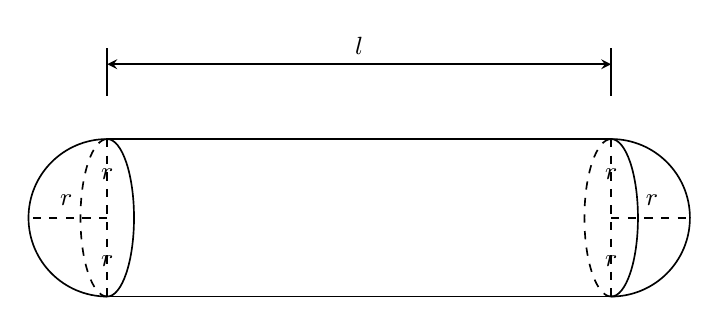
\begin{tikzpicture}[>=stealth, semithick, font=\small, x=1cm, y=1cm]
  \def\r{1.0}
  \def\L{6.4}
  \def\rx{0.34}
  % 圆柱母线
  \draw (0,\r) -- (\L,\r);
  \draw (0,-\r) -- (\L,-\r);
  % 两端半球的外轮廓
  \draw (0,\r) arc (90:270:\r);
  \draw (\L,-\r) arc (-90:90:\r);
  % 左端交线圆：左半实线、右半虚线
  \draw (0,\r) arc (90:-90:{\rx} and {\r});
  \draw[dashed] (0,-\r) arc (-90:-270:{\rx} and {\r});
  % 右端交线圆：左半实线、右半虚线
  \draw (\L,\r) arc (90:-90:{\rx} and {\r});
  \draw[dashed] (\L,-\r) arc (-90:-270:{\rx} and {\r});
  % 左端半径与直径
  \draw[dashed] (0,\r) -- (0,-\r);
  \draw[dashed] (0,0) -- (-\r,0);
  \node at (0,{0.55*\r}) {$r$};
  \node at (0,{-0.55*\r}) {$r$};
  \node at ({-0.52*\r},{0.22*\r}) {$r$};
  % 右端半径与直径
  \draw[dashed] (\L,\r) -- (\L,-\r);
  \draw[dashed] (\L,0) -- ({\L+\r},0);
  \node at (\L,{0.55*\r}) {$r$};
  \node at (\L,{-0.55*\r}) {$r$};
  \node at ({\L+0.52*\r},{0.22*\r}) {$r$};
  % 顶部标注 l
  \draw (\L,{\r+0.55}) -- (\L,{\r+1.15});
  \draw (0,{\r+0.55}) -- (0,{\r+1.15});
  \draw[<->] (0,{\r+0.95}) -- (\L,{\r+0.95});
  \node[above] at ({0.5*\L},{\r+0.95}) {$l$};
\end{tikzpicture}
\end{center}
\nopagebreak[4]
\Needspace{4\baselineskip}
\textbf{解析}
\gksubpart{(1)}
\Needspace{5\baselineskip}
圆柱部分体积 $\pi r^2l$，两端半球合起来是一个半径 $r$ 的球，体积 $\dfrac43\pi r^3$，故
\nopagebreak[4]
\[\pi r^2l+\frac43\pi r^3=\frac{80\pi}3\Longrightarrow 3r^2l+4r^3=80,\]
即 $l=\dfrac{80-4r^3}{3r^2}$。由 $l\geqslant2r$ 得 $80-4r^3\geqslant6r^3$，即 $r^3\leqslant8$，$0<r\leqslant2$。
\Needspace{5\baselineskip}
表面积中圆柱侧面积 $2\pi rl$，两端半球表面积合计 $4\pi r^2$，故
\nopagebreak[4]
\[y=3\cdot2\pi rl+c\cdot4\pi r^2=6\pi r\cdot\frac{80-4r^3}{3r^2}+4\pi cr^2
=\frac{160\pi}{r}-8\pi r^2+4\pi cr^2=\frac{160\pi}{r}+4\pi(c-2)r^2,\]
定义域 $0<r\leqslant2$。

\gksubpart{(2)}
\Needspace{5\baselineskip}
求导：
\nopagebreak[4]
\[y'=-\frac{160\pi}{r^2}+8\pi(c-2)r=\frac{8\pi[(c-2)r^3-20]}{r^2}.\]
令 $y'=0$ 得 $r^3=\dfrac{20}{c-2}$。因 $c>3$：
当 $3<c\leqslant4.5$ 时 $\dfrac{20}{c-2}\geqslant8$，临界点 $r\geqslant2$，在 $(0,2]$ 上 $y'<0$，$y$ 递减，最小值在 $r=2$；
当 $c>4.5$ 时临界点在 $(0,2)$ 内，$y$ 先减后增，最小值在 $r=\sqrt[3]{\dfrac{20}{c-2}}$。

\gkanswer{答案（1）：$y=\dfrac{160\pi}{r}+4\pi(c-2)r^2$，定义域 $0<r\leqslant2$。}

\gkanswer{答案（2）：$3<c\leqslant4.5$ 时 $r=2$；$c>4.5$ 时 $r=\sqrt[3]{\dfrac{20}{c-2}}$。}

\end{answer}
\begin{answer}
\gksolhead{22}{}

\textbf{题目}：

已知动直线 $l$ 与椭圆 $C:\dfrac{x^2}{3}+\dfrac{y^2}{2}=1$ 交于 $P(x_1,y_1)$，$Q(x_2,y_2)$ 两不同点，且 $\triangle OPQ$ 的面积 $S_{\triangle OPQ}=\dfrac{\sqrt6}{2}$，其中 $O$ 为坐标原点。

（1） 证明：$x_1^2+x_2^2$ 和 $y_1^2+y_2^2$ 均为定值；

（2） 设线段 $PQ$ 的中点为 $M$，求 $|OM|\cdot|PQ|$ 的最大值；

（3） 椭圆 $C$ 上是否存在三点 $D$，$E$，$G$，使得 $S_{\triangle ODE}=S_{\triangle ODG}=S_{\triangle OEG}=\dfrac{\sqrt6}{2}$？若存在，判断 $\triangle DEG$ 的形状；若不存在，请说明理由。

\Needspace{4\baselineskip}
\textbf{解析}
作伸缩变换 $u=\dfrac{x}{\sqrt3}$，$v=\dfrac{y}{\sqrt2}$，椭圆变为单位圆 $u^2+v^2=1$，面积放大 $\sqrt6$ 倍。故 $S_{\triangle OPQ}=\dfrac{\sqrt6}2$ 等价于变换后 $S_{\triangle OP'Q'}=\dfrac12$。
\Needspace{5\baselineskip}
对单位圆上两点，$S=\dfrac12|u_1v_2-u_2v_1|=\dfrac12$，故 $|u_1v_2-u_2v_1|=1$，即两向量垂直：$u_1u_2+v_1v_2=0$，亦即在原坐标中
\nopagebreak[4]
\[\frac{x_1x_2}{3}+\frac{y_1y_2}{2}=0\Longrightarrow 2x_1x_2+3y_1y_2=0.\]

\gksubpart{(1)}
\Needspace{5\baselineskip}
在单位圆中令 $P'=(\cos\alpha,\sin\alpha)$，$Q'=(-\sin\alpha,\cos\alpha)$。则
\nopagebreak[4]
\[u_1^2+u_2^2=\cos^2\alpha+\sin^2\alpha=1,\qquad v_1^2+v_2^2=\sin^2\alpha+\cos^2\alpha=1,\]
\Needspace{5\baselineskip}
故
\nopagebreak[4]
\[x_1^2+x_2^2=3(u_1^2+u_2^2)=3,\qquad y_1^2+y_2^2=2(v_1^2+v_2^2)=2,\]
均为定值。

\gksubpart{(2)}
\Needspace{5\baselineskip}
中点 $M'$ 的坐标 $m_u=\dfrac{\cos\alpha-\sin\alpha}{2}$，$m_v=\dfrac{\sin\alpha+\cos\alpha}{2}$。记 $s=\sin2\alpha$，则
\nopagebreak[4]
\[|OM|^2=3m_u^2+2m_v^2=\frac{5-s}{4},\qquad |PQ|^2=3(\cos\alpha+\sin\alpha)^2+2(\sin\alpha-\cos\alpha)^2=5+s.\]
\Needspace{5\baselineskip}
于是
\nopagebreak[4]
\[(|OM|\cdot|PQ|)^2=\frac{(5-s)(5+s)}4=\frac{25-s^2}{4}\leqslant\frac{25}4,\]
当 $s=0$ 时取等，故 $|OM|\cdot|PQ|$ 的最大值为 $\dfrac52$。

\gksubpart{(3)}
若存在三点 $D,E,G$ 使三个三角形面积都等于 $\dfrac{\sqrt6}2$，则在单位圆中任意两点与圆心组成的三角形面积都是 $\dfrac12$，故任意两点的位置向量都垂直。但平面上不存在三个两两垂直的非零向量（第三个只能与其中一个共线），矛盾。因此不存在这样的三点。

\gkanswer{答案（1）：证明见解析，$x_1^2+x_2^2=3$，$y_1^2+y_2^2=2$。}

\gkanswer{答案（2）：最大值 $\dfrac52$。}

\gkanswer{答案（3）：不存在。}

\end{answer}